\documentclass[aspectratio=169, 12pt]{beamer}

\usepackage{lmodern}
\usepackage{hyperref}
\usepackage{graphicx}
\usepackage{booktabs}
\usepackage[authordate,maxcitenames=1,backend=biber,doi=false,isbn=false,url=false]{biblatex-chicago}
\renewcommand*{\nameyeardelim}{\addcomma\addspace}
% \addbibresource{discrimination.bib}

\usepackage{amsmath}
\usepackage{amssymb}
\usepackage{amsthm}
\usepackage{bm}
\usepackage{bbm}
\usepackage{mathtools}
\setbeamertemplate{theorems}[numbered]
\newtheorem{proposition}{Proposition}
\newtheorem{assumption}{Assumption}

\DeclareMathOperator*{\plim}{plim}
\DeclareMathOperator*{\var}{var}
\DeclareMathOperator*{\cov}{cov}

\newcommand{\indep}{\perp \!\!\! \perp}
\newcommand{\R}{\mathbb{R}}
\newcommand{\I}{\mathbbm{1}}
\newcommand{\argmax}{\mathop{\rm arg~max}\limits}
\newcommand{\argmin}{\mathop{\rm arg~min}\limits}

% preambles for tables
\usepackage{booktabs}
\usepackage{adjustbox}
\usepackage{caption}
\captionsetup{labelformat=empty}
\usepackage{tikz}
\usetikzlibrary{calc}
\newcommand{\tikzmark}[1]{\tikz[overlay,remember picture] \node (#1) {};}
\newcommand{\DrawBox}[1][]{%
    \tikz[overlay,remember picture]{
    \draw[#1,thick]
      ($(left)+(-0.2em,0.9em)$) rectangle
      ($(right)+(0.2em,-0.3em)$);}
}
\usepackage[group-separator={,}]{siunitx}
\usepackage{longtable}
\usepackage{rotating}
\usepackage{threeparttable}

\newcommand{\backupbegin}{
   \newcounter{framenumberappendix}
   \setcounter{framenumberappendix}{\value{framenumber}}
}
\newcommand{\backupend}{
   \addtocounter{framenumberappendix}{-\value{framenumber}}
   \addtocounter{framenumber}{\value{framenumberappendix}} 
}

\usepackage{silence}
\WarningFilter{latexfont}{Font shape}
\WarningFilter{biblatex}{Patching footnotes failed}

\usetheme{Boadilla}
\usecolortheme{orchid}
\usefonttheme{professionalfonts}

\setbeamertemplate{section in toc}[sections numbered]
\setbeamertemplate{itemize item}[default]
\setbeamertemplate{itemize subitem}[square]
\setbeamertemplate{enumerate items}[default]
\setbeamertemplate{navigation symbols}{}
\setbeamertemplate{itemize/enumerate body begin}{\normalsize}
\setbeamertemplate{itemize/enumerate subbody begin}{\normalsize}
\setbeamertemplate{itemize/enumerate subsubbody begin}{\normalsize}
\setbeamerfont{title}{size=\large}
\setbeamerfont{institute}{size=\small}
\setbeamercovered{dynamic}


\title[Shimizuguchi et al. (2020, Cancer)]{Shimizuguchi et al. (2020, Cancer)}
\author[Konan Hara]{Konan Hara}
\institute[Arizona]{University of Arizona}
\date{\today}
\begin{document}

	% \begin{frame}[plain]
	% \titlepage
	% \end{frame}

	\begin{frame}
	\frametitle{Shimizuguchi et al. (2020, Cancer)}
	\centering{
	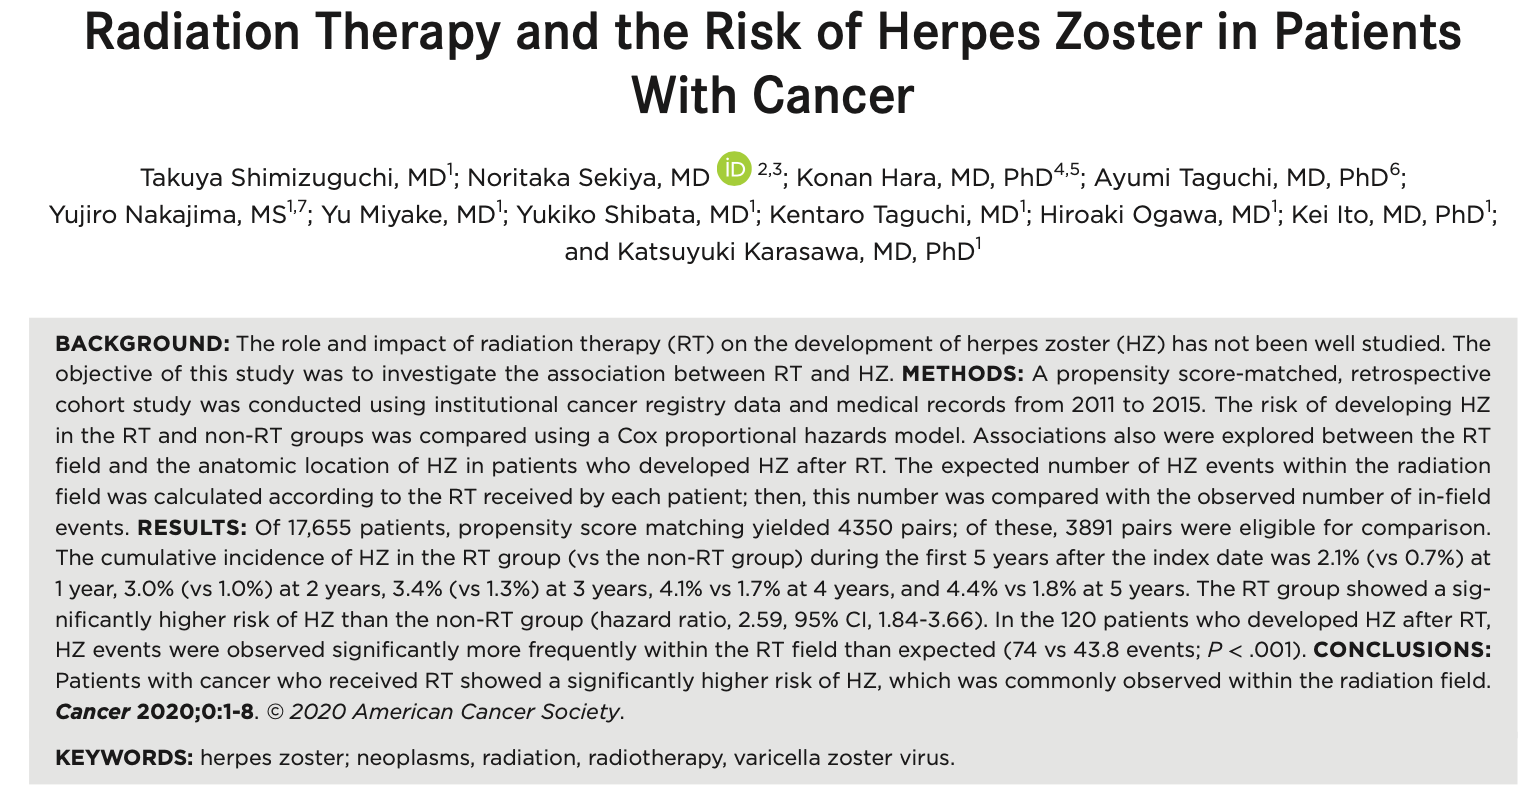
\includegraphics[width=\textwidth]{fig/Shimizuguchi_front.png}
	}
	\end{frame}

	\begin{frame}
	\frametitle{Introduction}
	\begin{itemize}
	\item Several studies have investigated the development of herpes zoster (HZ) after radiation therapy (RT) and have described the frequency and timing of events and the clinical course.
	\item However, most of those studies were limited to cohorts of patients with a specific malignant disease and lacked robust statistical analyses.
	\item We assessed the relation between receipt of RT and the development of HZ in patients with cancer using a 2-pronged approach:
	\begin{enumerate}
	\item we compared the prevalence of HZ in propensity score-matched RT and non-RT recipients;
	\item \textcolor{red}{we assessed whether the anatomic location of an HZ event was related to the radiation field}.
	\end{enumerate}

	\end{itemize}
	\end{frame}

	\begin{frame}
	\frametitle{Problem of Survival Analysis With Matching---Lead-time Bias}
	\centering{
	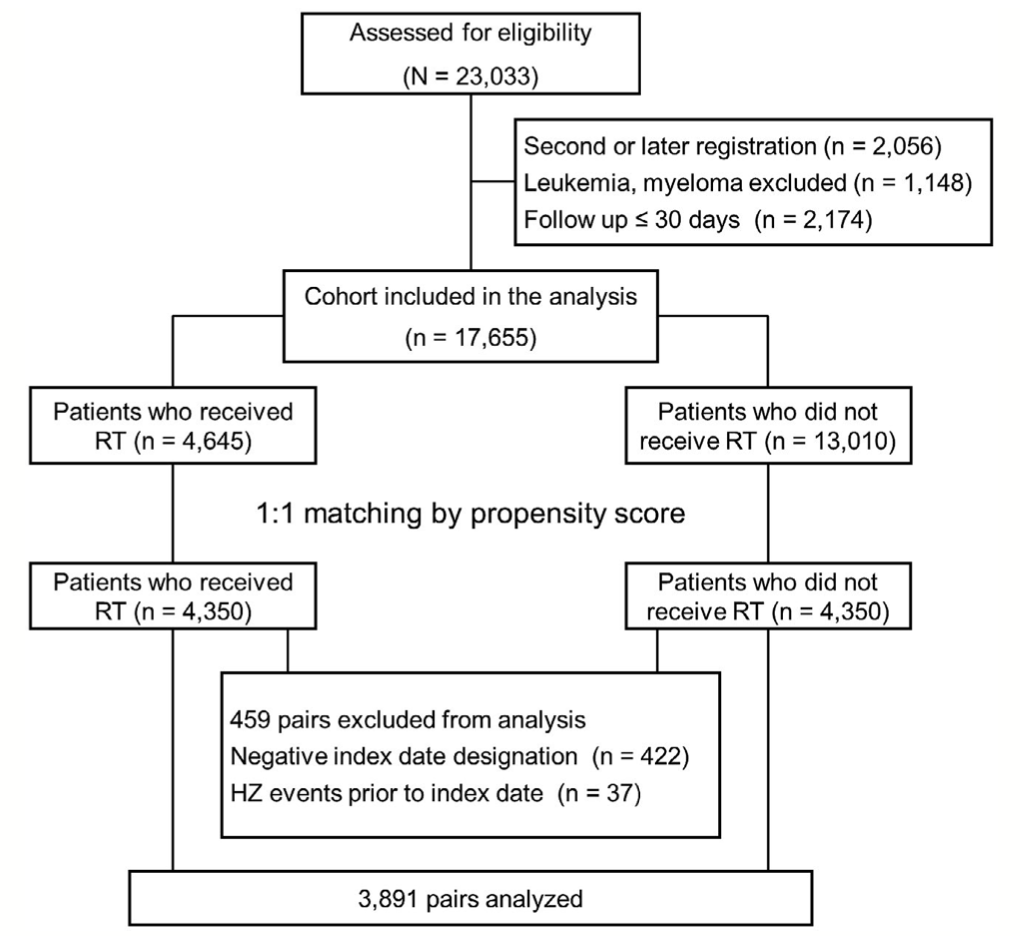
\includegraphics[width=0.55\textwidth]{fig/Shimizuguchi_fig1.png}
	}
	\end{frame}

	\begin{frame}
	\frametitle{Comparison of RT Field and Anatomic Location of HZ}
	\begin{itemize}
	\item Theoretically, we can state that the irradiated body area is related to the body area affected by an HZ event if a difference exists between the marginal distribution of the body area affected by HZ events and its distribution conditional on the irradiated body area.
	\item To implement this idea empirically, we devised a simple statistical test for all eligible patients who received RT before the development of HZ. 
	\item We computed the marginal probability of an HZ event occurring on the irradiated body area from the empirical marginal distribution of the 5 anatomic body areas (trigeminal, cervical, thoracic, lumbar, and caudal) affected by HZ events.

	\end{itemize}
	\end{frame}

	\begin{frame}
	\frametitle{Empirical Marginal Distribution of Body Area Affected by HZ}
	\begin{itemize}
	\item We categorized the body surface into 64 mutually exclusive parts based on spinal cord segments: bilateral trigeminal 1–3, cervical 2–8, thoracic 1–12, lumbar 1–5, and sacral 1–5.
	\item Each HZ event was categorized into the most appropriate segment according to the affected dermatomal location. 
	\item The empirical marginal distribution of the body area affected by HZ events was calculated as an empirical probability mass function of an HZ event occurrence on any of the 64 segments. 
	\item Because of the scarcity of data, we imposed the probability of an HZ event occurrence per segment to be the same within five large anatomical groups: trigeminal, cervical, thoracic, lumbar, and sacral. 

	\end{itemize}
	\end{frame}

	\begin{frame}
	\frametitle{Empirical Marginal Distribution of Body Area Affected by HZ}
	Probability of an HZ event occurrence on segment $s$, $\Pr(s)$, was calculated as follows:
	\begin{eqnarray*}
	\Pr(s) = \frac{n_g}{N} \times \frac{1}{d_g}
	\end{eqnarray*}
	\begin{itemize}
	\item $g$ is an anatomical group that includes segment $s$
	\item $n_g$ is the observed number of HZ events categorized into group $g$
	\item $N$ is the total number of HZ events
	\item $d_g$ is the number of dermatome segments included in group $g$

	\end{itemize}
	\end{frame}

	\begin{frame}
	\centering{
	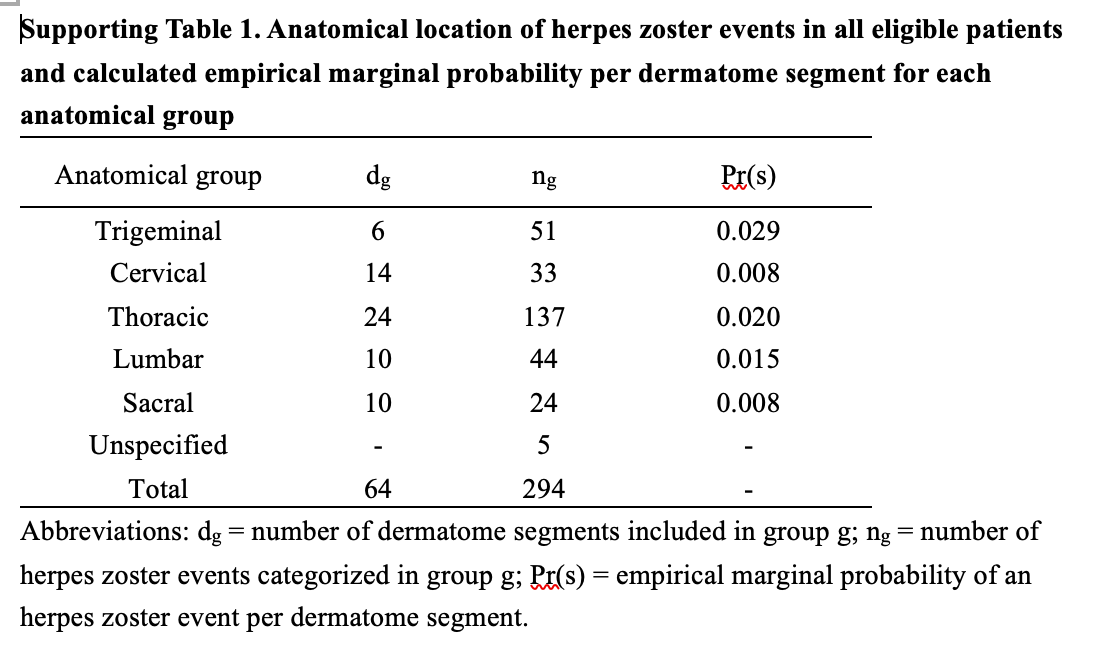
\includegraphics[width=0.9\textwidth]{fig/Shimizuguchi_tabS1.png}
	}
	\end{frame}

	\begin{frame}
	\frametitle{Comparison of RT Field and Anatomic Location of HZ Events}
	\begin{itemize}
	\item A post-RT HZ event was categorized as an in-field event if it occurred in the radiation field or as an out-field event otherwise.
	\item If the null hypothesis (the irradiated body area is unrelated to the body area affected by HZ events) were true, then the totaled marginal probability of in-field events can be considered as the expected number of in-field events in the cohort.
	\item We can test the null hypothesis by comparing this value with the observed number of in-field events.

	\end{itemize}
	\end{frame}

	\begin{frame}
	\centering{
	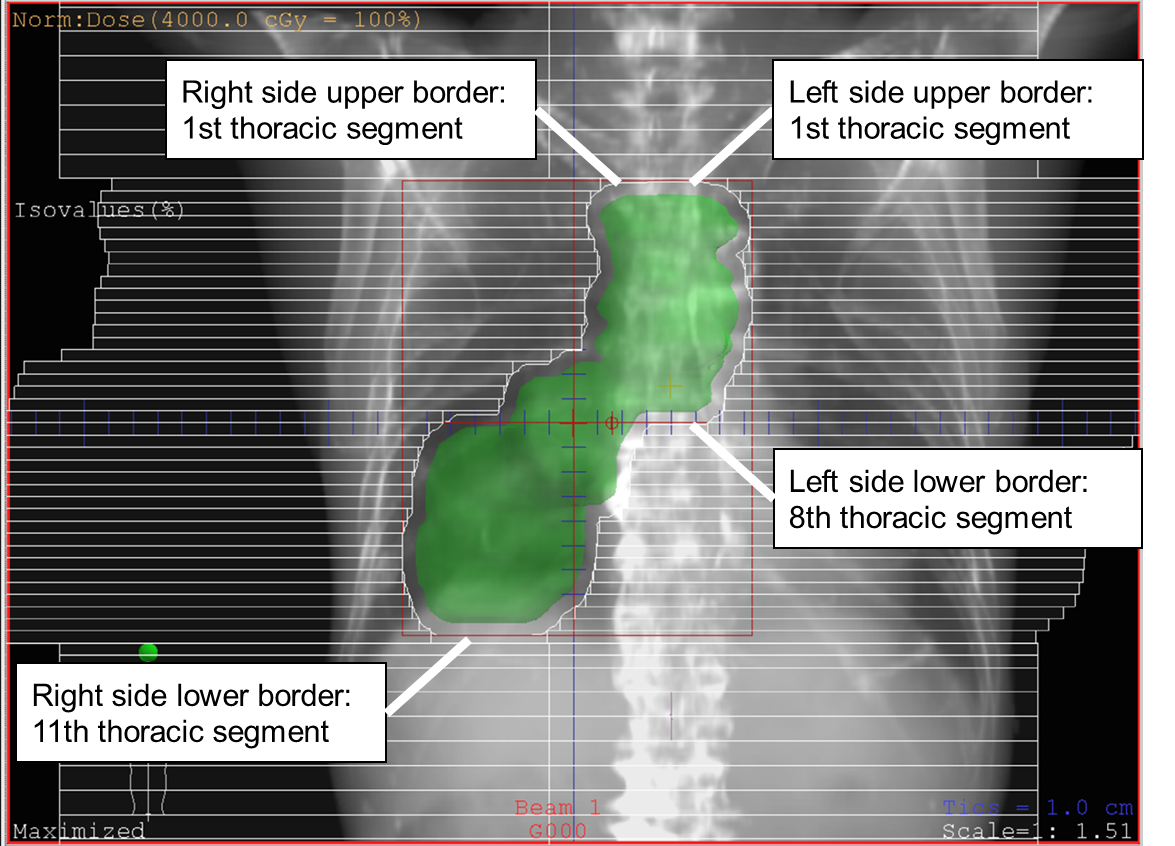
\includegraphics[width=0.9\textwidth]{fig/Shimizuguchi_figS1.png}
	}
	\end{frame}

	\begin{frame}
	\frametitle{Statistical Testing}
	\centering{
	
\includegraphics[width=0.6\textwidth]{fig/Bivand_front.png}
	}
	\end{frame}

	\begin{frame}
	\frametitle{Disease Mapping}
	\centering{
	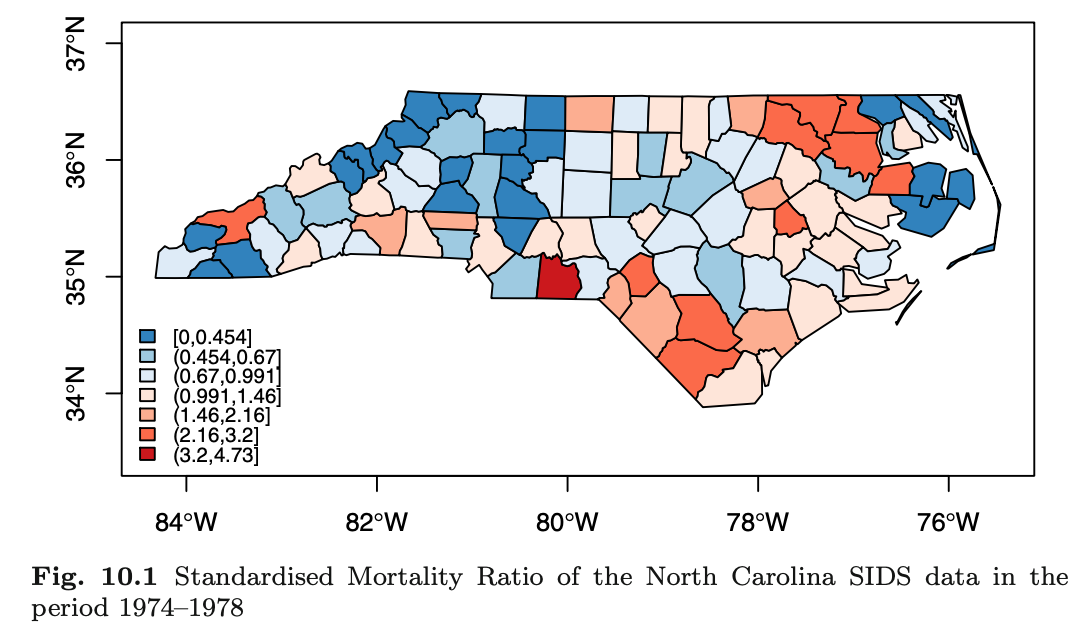
\includegraphics[width=0.8\textwidth]{fig/Bivand_fig10_1.png}
	}
	\end{frame}

	\begin{frame}
	\frametitle{Testing the Homogeneity of the Relative Risks\footnote{Bivand, Pebesma, and Gomez-Rubio Section 10.6.1}}
	\begin{itemize}
	\item Disease mapping provides a first insight to the spatial distribution of the disease but it may be required to locate the presence of zones where the risk tends to be unusually higher than expected.
	\item We can test whether there are actual differences among the different relative risks.
	\item Given that for each area we have computed its expected and observed number of cases ($O_i$, observed; $E_i$, expected), a chi-square test can be carried out to test for (global) significant differences between these two quantities:
	\begin{eqnarray*}
	\chi^2 = \sum_{i=1}^n \frac{(O_i-E_i)^2}{E_i} \overset{a}{\sim} \chi^2_{n-1}
	\end{eqnarray*}
	\begin{itemize}
	\item internal standardization is used to obtain $E_i$: $\sum_{i=1}^n O_i = \sum_{i=1}^n E_i $
	\end{itemize}

	\end{itemize}
	\end{frame}

	\begin{frame}
	\frametitle{Results: RT and Anatomic Distribution of HZ Events}
	\begin{itemize}
	\item The total number of HZ events in the 17,655 eligible patients was 294, which was used to calculate the empirical marginal probability of HZ events.
	\item Of 294 events, 123 were observed after RT, and 120 of those (3 events were excluded because of unspecified HZ distribution) were used to test the null hypothesis.
	\item The expected number of in-field versus out-field HZ events under the null hypothesis for the 120 patients was 43.8 versus 76.2 events, respectively.
	\item The observed number of in-field versus out-field HZ events was 74 versus 46 events, respectively, which was significantly higher than the expected number of in-field HZ events ($P < .001$).

	\end{itemize}
	\end{frame}













\end{document}
